% mn2esample.tex
%
% v2.1 released 22nd May 2002 (G. Hutton)
%
% The mnsample.tex file has been amended to highlight
% the proper use of LaTeX2e code with the class file
% and using natbib cross-referencing. These changes
% do not reflect the original paper by A. V. Raveendran.
%
% Previous versions of this sample document were
% compatible with the LaTeX 2.09 style file mn.sty
% v1.2 released 5th September 1994 (M. Reed)
% v1.1 released 18th July 1994
% v1.0 released 28th January 1994

\documentclass[useAMS,usenatbib]{mn2e}

% If your system does not have the AMS fonts version 2.0 installed, then
% remove the useAMS option.
%
% useAMS allows you to obtain upright Greek characters.
% e.g. \umu, \upi etc.  See the section on "Upright Greek characters" in
% this guide for further information.
%
% If you are using AMS 2.0 fonts, bold math letters/symbols are available
% at a larger range of sizes for NFSS release 1 and 2 (using \boldmath or
% preferably \bmath).
%
% The usenatbib command allows the use of Patrick Daly's natbib.sty for
% cross-referencing.
%
% If you wish to typeset the paper in Times font (if you do not have the
% PostScript Type 1 Computer Modern fonts you will need to do this to get
% smoother fonts in a PDF file) then uncomment the next line
% \usepackage{Times}

%%%%% AUTHORS - PLACE YOUR OWN MACROS HERE %%%%%
\usepackage{subfigure}
\usepackage{amsmath}	% Advanced maths commands
\usepackage{amssymb}	% Extra maths symbols
\usepackage{graphicx}
\newcommand{\bz}{\bmath{z}}
\newcommand{\br}{\bmath{r}}
\newcommand{\bg}{\bmath{g}}
\newcommand{\bd}{\bmath{d}}
\newcommand{\bv}{\bmath{v}}
\newcommand{\bn}{\bmath{n}}
\newcommand{\by}{\bmath{y}}
\newcommand{\bJ}{\bmath{J}}
\newcommand{\bD}{\bmath{D}}
\newcommand{\conj}[1]{\overline{#1}}
%%%%%%%%%%%%%%%%%%%%%%%%%%%%%%%%%%%%%%%%%%%%%%%%

\title[Dust envelopes around RV Tauri stars]{Dust envelopes around RV Tauri stars}
\author[A. V. Raveendran and A. N. Other]{A. V. Raveendran$^{1}$\thanks{E-mail:
email@address (AVR); otheremail@otheraddress (ANO)} and A. N.
Other$^{2}$\footnotemark[1]\thanks{This file has been amended to
highlight the proper use of \LaTeXe\ code with the class file.
These changes are for illustrative purposes and do not reflect the
original paper by A. V. Raveendran.}\\
$^{1}$Indian Institute of Astrophysics, Bangalore 560034, India\\
$^{2}$Building, Institute, Street Address, City, Code, Country}
\begin{document}

\date{Accepted 1988 December 15. Received 1988 December 14; in original form 1988 October 11}

\pagerange{\pageref{firstpage}--\pageref{lastpage}} \pubyear{2002}

\maketitle

\label{firstpage}

\begin{abstract}
In the {\it IRAS\/} [12]--[25],  [25]--[60] colour--colour diagram, RV
Tauri stars are found to populate cooler temperature regions
$(T<600\,\rmn{K})$, distinctly different from those occupied by  the
oxygen and carbon Miras. The {\it IRAS\/} fluxes are  consistent with the
dust density in the envelope varying as the inverse square of the
radial distance, implying that the grain formation processes in these
objects are most probably continuous and not sporadic. It is found that
the spectroscopic subgroups A and B are well separated in the
far-infrared two-colour diagram, with group B objects having
systematically cooler dust envelopes. We interpret this as being due to
a difference in the nature of grains, including the chemical
composition, in the two cases.
\end{abstract}

\begin{keywords}
circumstellar matter -- infrared: stars.
\end{keywords}

\section{Introduction}

Main contributions of the paper:

\begin{enumerate}
 \item Present a general framework which unifies all the techniques developed so far showing they are all related (LINCAL, non-linear estimator, etc ...). They are all non-linear
 least-squares techniques, i.e. they either employ Gauss-Newton or the Levenberg-Marquardt algorithms. We have to start with LINCAL showing that it is GN, then we have to motivate 
 why we want to use Oleg's complex optimization framework.
 \item Use Oleg's complex optimization framework to re-derive the non-linear technique proposed by Marthi and Chengular. The novelty lies, in the fact that by using Oleg's
 framework we can find analytic expressions for the Jacobian, the Hessian and the Jacobian-residual product (which is not even the case for LINCAL). State that the algorithm is 
 effectively related to SteFCal and is eff an independent rediscovery of SteFCal and an extension of it into the redundant domain.
 \item Also we present the array geometry function to help us make the derivations from Marthi and Chengular easier to read and understand for a general layout.
 \item We also mention at this point that in Oleg's paper the question is raised is there a fast way of computing the exact inverse, we then present this new method, which is called
 conjugate gradient method. We discuss the algorithm and the two things which bound its execution time. Which is $kappa$ and $m$ (spectral condition number and its sparsity). Then
 we explore both of these parameters.
 \end{enumerate}
 
 **************
 FLOW OF PAPER
 **************
 
 \begin{enumerate}
 \item We need the definition of visibilities as in Liu. DEFINE SNR HERE ALREADY together maybe with the sigma value of the noise.
 \item Introduce the array geometery function.
 \item Write down logcal and lincal in matrix form... ?
 \item Short discussion of least squares and jacobian and hessian's. General GN and LM update rules.
 \item Introduce redundant calibration as a least squares problem. We will use this general fact to derive both popular methods.
 \item Propose a possible solution witch leads to lincal. Mention that this approach works as in this form the function is differentiable (a taylor expansion in the 
 parameters exists). Maybe mention that we can also divide the problem into real and imaginary etc...
 \item Show how this relates to lincal for example ---> show lincal is GN.
 \item Now introduce complex optimization ---> Main motivation for switching to the alternative framework is that the the differentials are very simplistic. We wish to show that
 we can derive the method of Chengular.
 \item Do the derivation of Chengular. 
 \item Brief discussion abouth Chengular and SteFCal and Complex Optimization. Here I show that in Oleg's paper he re-derives an algorithm called SteFCal. Stefcal works
 on the basis of alternating direction implicit method. The first signs of achieving a similar algorithm already appeared in Stefan's conference paper in which the alternating
 idea was first proposed. Then I mention Chegular re-derives the expression by using partial derivatives and extends it to redundant. One could also have used the linear alternating
 approach. In an attempt to merge the terminology that has independently develop in the general calibration and redundant calibration literature and to emphasize the close
 relationship between Stefcal and the approach derived by I will use the label Redunandat SteFCal (R-Stefcal) to refer to the NLS method proposed by ... Lastly we mention that similarly
 to how Oleg re-derived stefcal in, we have achieved the same approach.
 \item Faster Exact inverse. A question that Oleg poses in his paper is, does there exist a faster way to take the exact inverse of JhJ? One that is almost linear, and
 implies that we can therefore implement the full LM algorithm. The aim here is of course to reduce the number of iterations that are required to converge by using the 
 full inverse instead which would hopefully provide enough of a speedup to compensate for the more expensive full-inverse. The algorithm we propose is the conjugate 
 gradient method.
 \item We give the images of the HESSIAN of both lincal and the complex method (number of terms). So we can mention that both are sparse and contain diagonal entries that 
 are more significant than the off-diagonal entries. What linear inversion approach can take advantage of both these phenomenon. One such technique is 
 cg. 
 \item Briefly discuss CG and how its computationally bounded by its condition number and its sparsity (how does the diagonal play a role).
 \item Simulation description
 \item Will CG improve things?
 \item Now first discuss the condition
 number of the Hessian before and after pre-conditioning (pre-codnitioning can only be applied if a good inverse of a matrix is known, if it is known then it can improve 
 the spectral condition number of a matrix. We present here the kappa and iteration number graphs for the HEXAGONAL layout. Although the
 \item Now we discuss the sparsity results. 
 \item Provide a table that theoretical compares R-StEFCal and SPARC.
 \item Number of outerloop iterations. 
 \item Timing results.
 \item Accuracy results.
 \item Maybe some freq simulations.
 \end{enumerate}
 
 We
 
 \section{Visibilities}
The observed visibility $d_{pq}$ measured by the baseline formed by antenna $p$ and $q$ can be described as

\begin{equation}
\label{eq:vis_definition}
d_{pq} = g_{p}\conj{g}_{q}y_{pq} + n_{pq},
\end{equation}
where $g_{p}$ and $g_{q}$ are the direction independent gains associated with antenna $p$ and $q$, $y_{pq}$ denotes the true visibility that baseline $pq$ measured
and $n_{pq}$ is the thermal noise component. Conjugation is denoted by $\conj{(*)}$. During the course of an actual observation the true value of $g_p$, $g_q$ and $y_{pq}$ are unknown and are the quantities which infact have 
to be estimated.

The real and imaginary components of the thermal noise is normally distributed with a mean of zero and a standard deviation that is equal to [NB - are the real and imaginary parts defined with same sigma?]  
\begin{equation}
\sigma = \frac{\sqrt{2}k_{B}T_{\textrm{sys}}}{A\eta\sqrt{\Delta \nu \tau}}, 
\end{equation}
where $k_B$ is Boltzmann's constant, $T_{\textrm{sys}}$ is equal to the system temperature, $A$ is the effective collecting area of each element in the array, $\eta$ is a dimensionless
efficiency factor, $\Delta \nu$ is the observational bandwidth and $\tau$ is the integration time per visibility. 

\subsection{Redundant Array Geometry Mapping}
If an array is redundant then its redundant baselines sample the exact same visibilites in the $uv$-plane, i.e. if baseline $pq$ and $rs$ are redundant then $y_{pq} = y_{rs}$. We can
therefore also use the following useful indexing strategy: We can use singular redundant baseline indexes instead of composite antenna pairs to label the true observed visibilities. 

Let $\phi_{ij}:\mathbb{N}^2\rightarrow\mathbb{N}^+$ be the mapping that maps composite antenna pairs to the unique redundant baseline indexes of an array. This mapping is not symmetric as 
$\phi_{ij} = 0$ if $i>j$. It is possible to construct a simple analytic expression for $\phi_{ij}$ when our array is in an east-west regular configuration:
\begin{equation}
\phi_{ij} = 
\begin{cases}
j-i&\textrm{if}~i<j\\
0&\textrm{otherwise}
\end{cases}.
\end{equation}
It becomes increasingly more difficult to construct analytic expressions of $\phi_{ij}$ for other more complicated array layouts.

We can also define the following symmetric variant of $\phi_{ij}$:
\begin{equation}
\zeta_{ij} = 
\begin{cases}
\phi_{ij}~\textrm{if}~i\leq j\\
\phi_{ji}~\textrm{if}~i>j
\end{cases}.
\end{equation} 

\begin{figure*}
\centering
\subfigure[full-complex:   Real]
{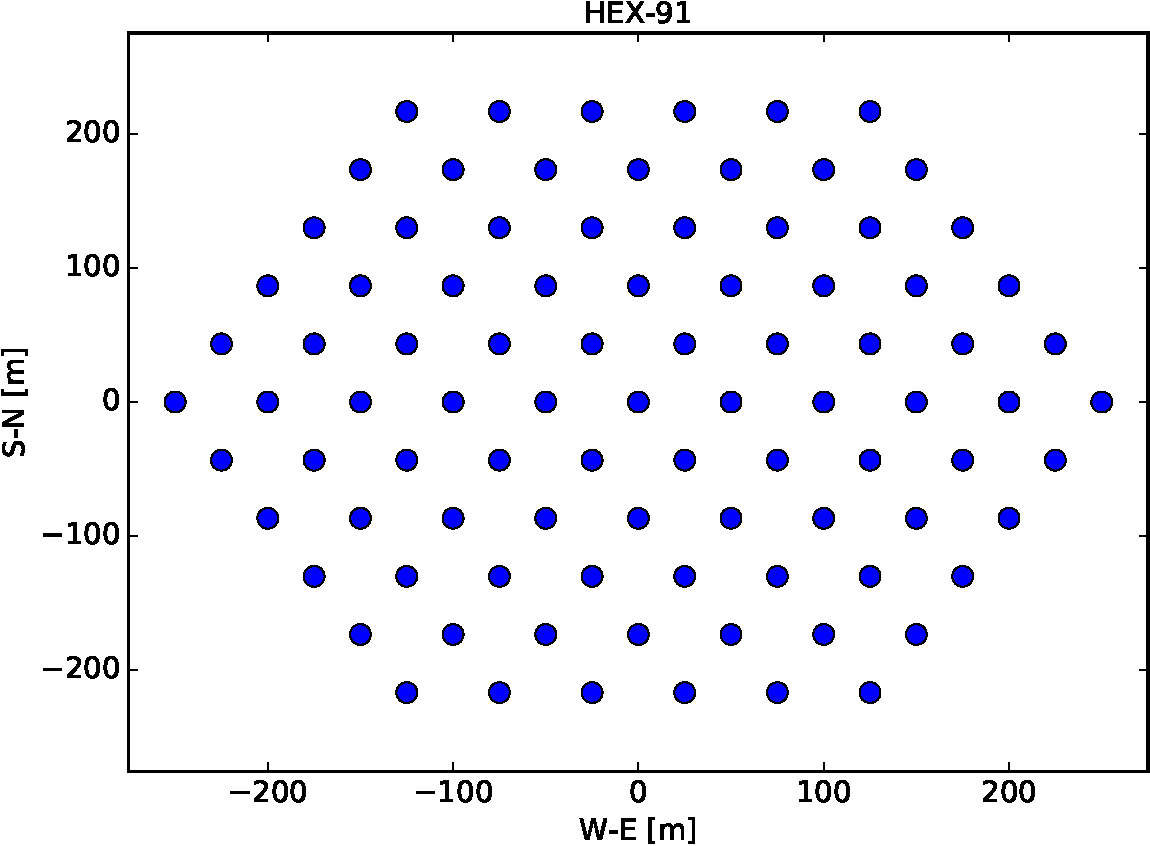
\includegraphics[width=0.33\textwidth]{./HEX_lay.pdf}\label{fig:stef_r}}
\subfigure[full-complex:  Imag]
{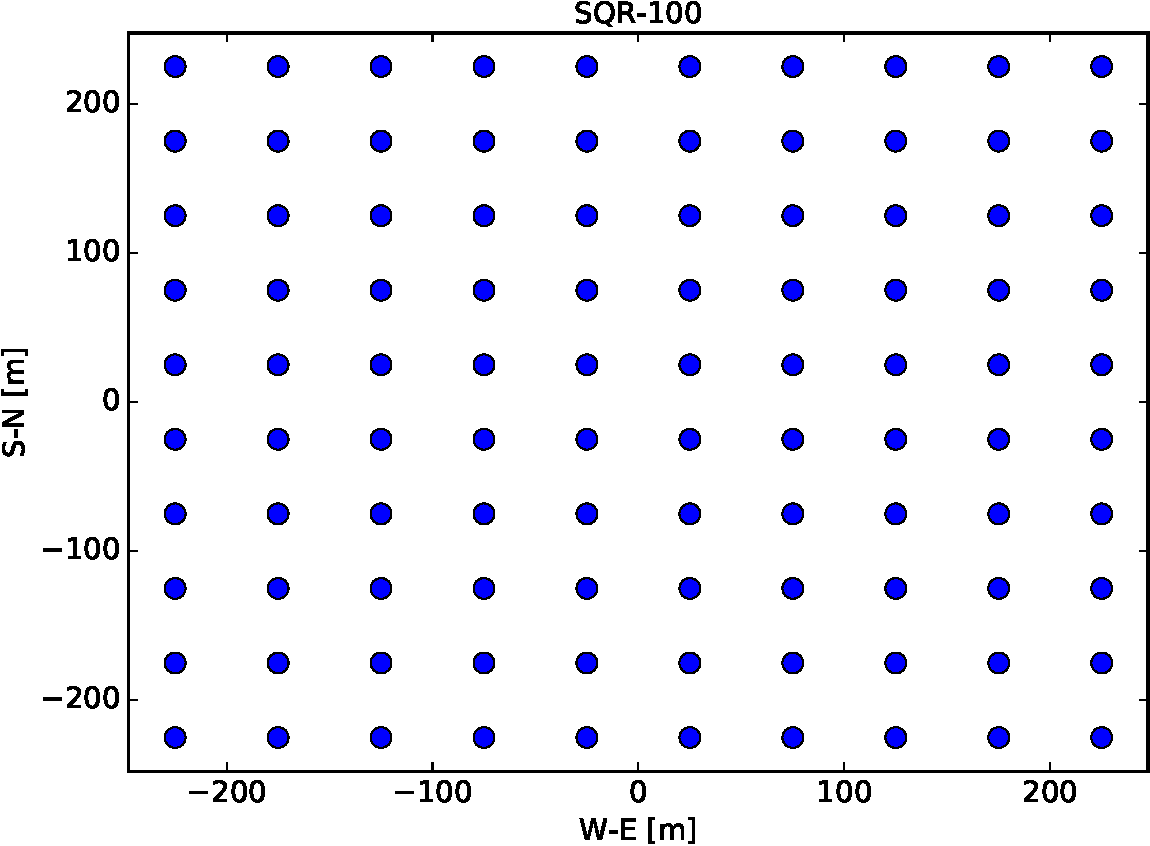
\includegraphics[width=0.33\textwidth]{./SQR_lay.pdf}\label{fig:stef_i}}
\subfigure[full-complex: ghost pattern]
{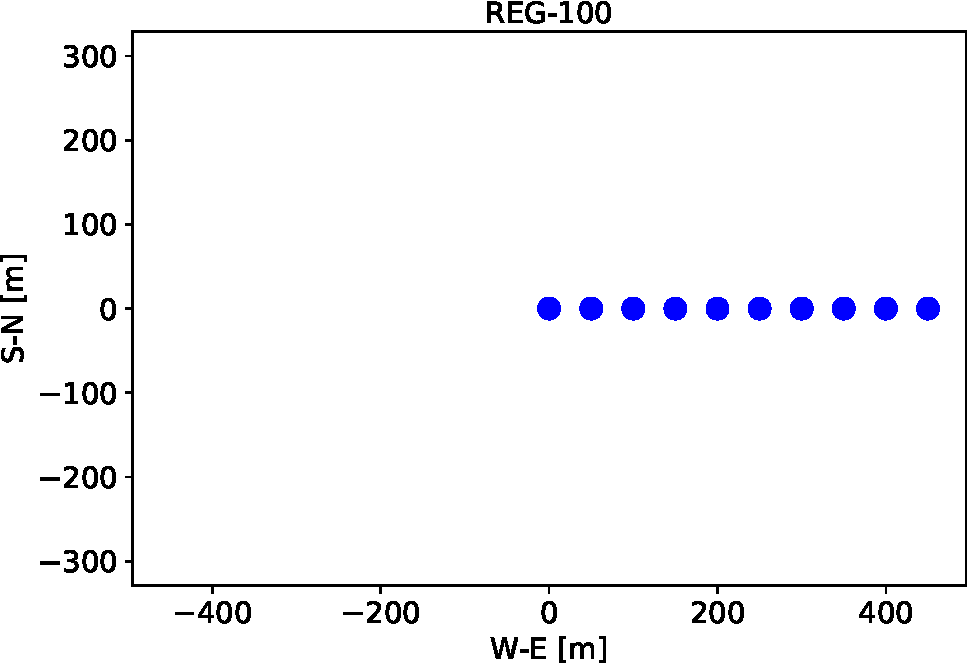
\includegraphics[width=0.33\textwidth]{./REG_lay.pdf}\label{fig:full_pat_45}}

\subfigure[phase-only:   Real]
{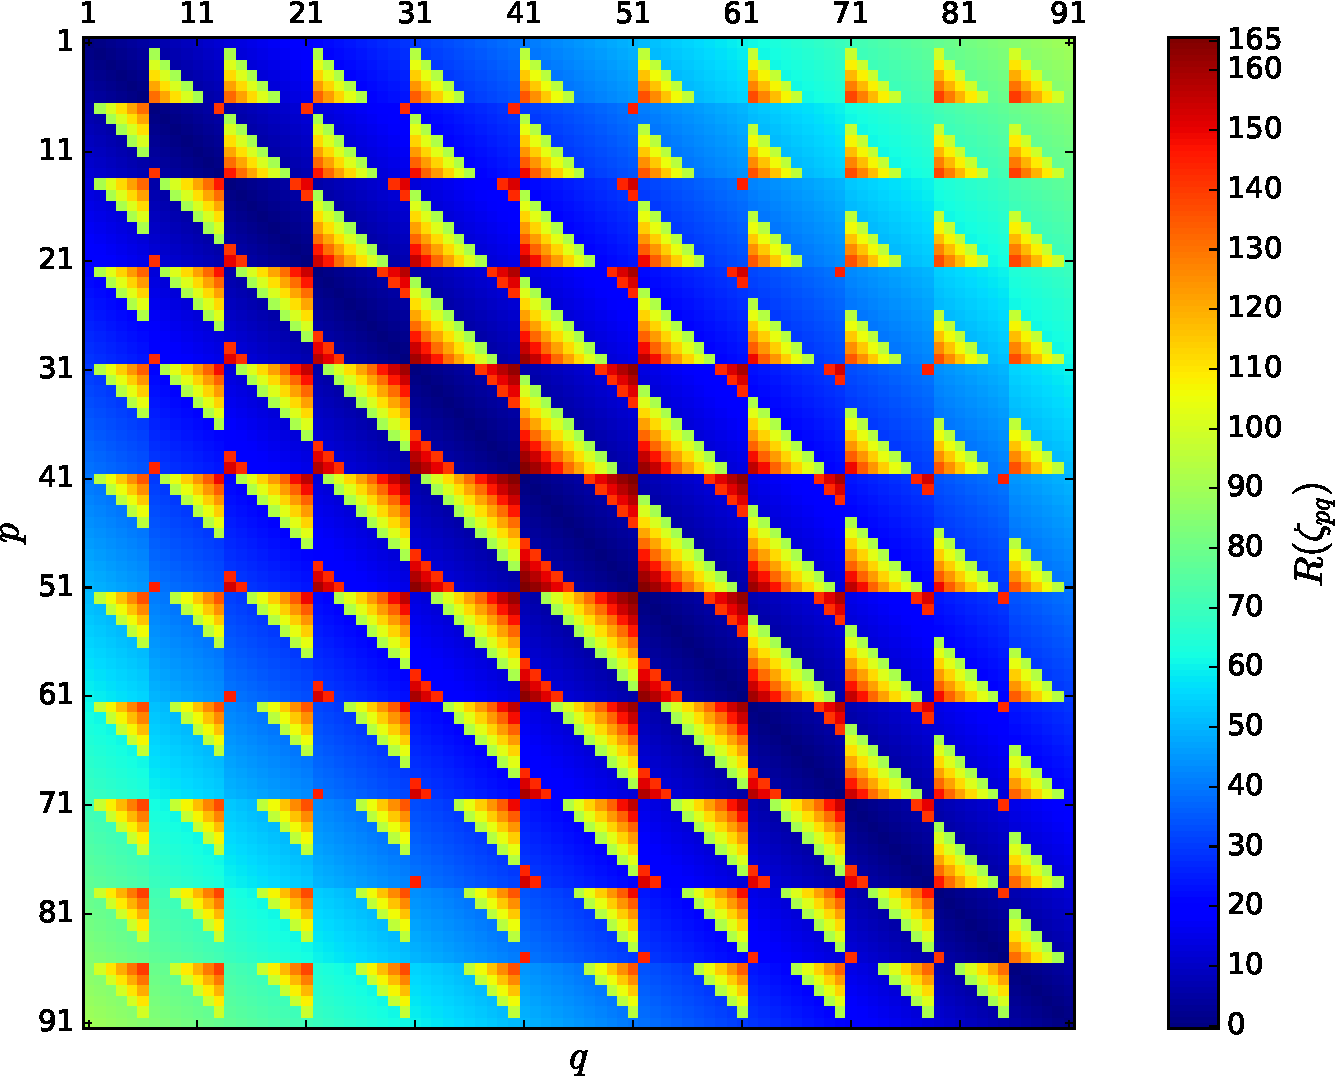
\includegraphics[width=0.33\textwidth]{./HEX_phi.pdf}\label{fig:phase_r}}
\subfigure[phase-only:   Imag]
{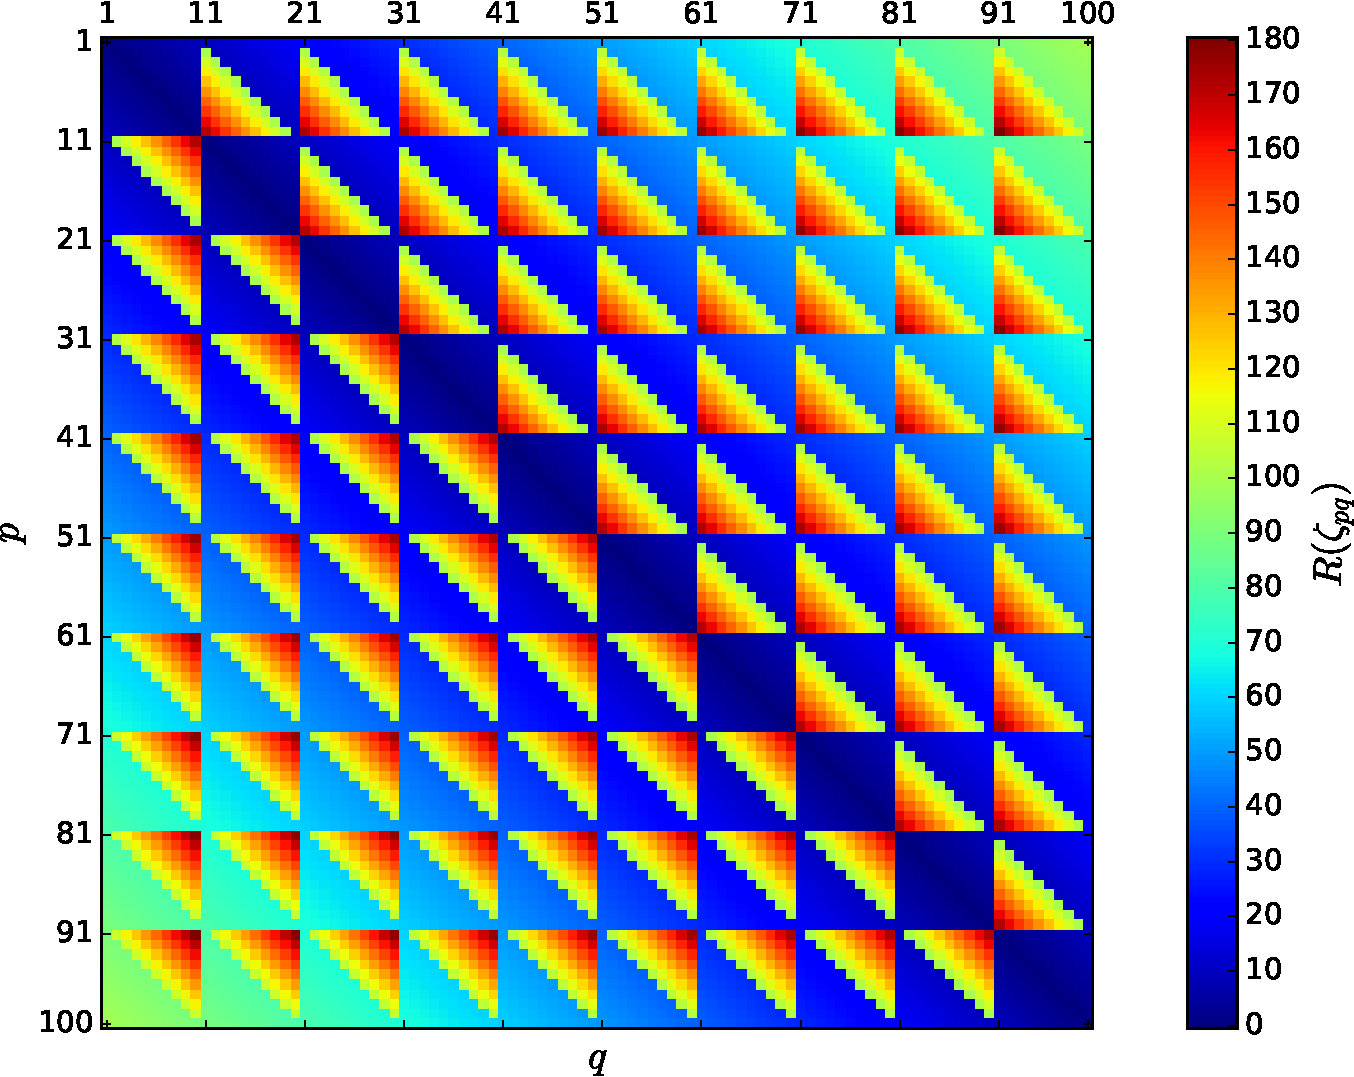
\includegraphics[width=0.33\textwidth]{./SQR_phi.pdf}\label{fig:phase_i}}
\subfigure[phase-only: ghost pattern]
{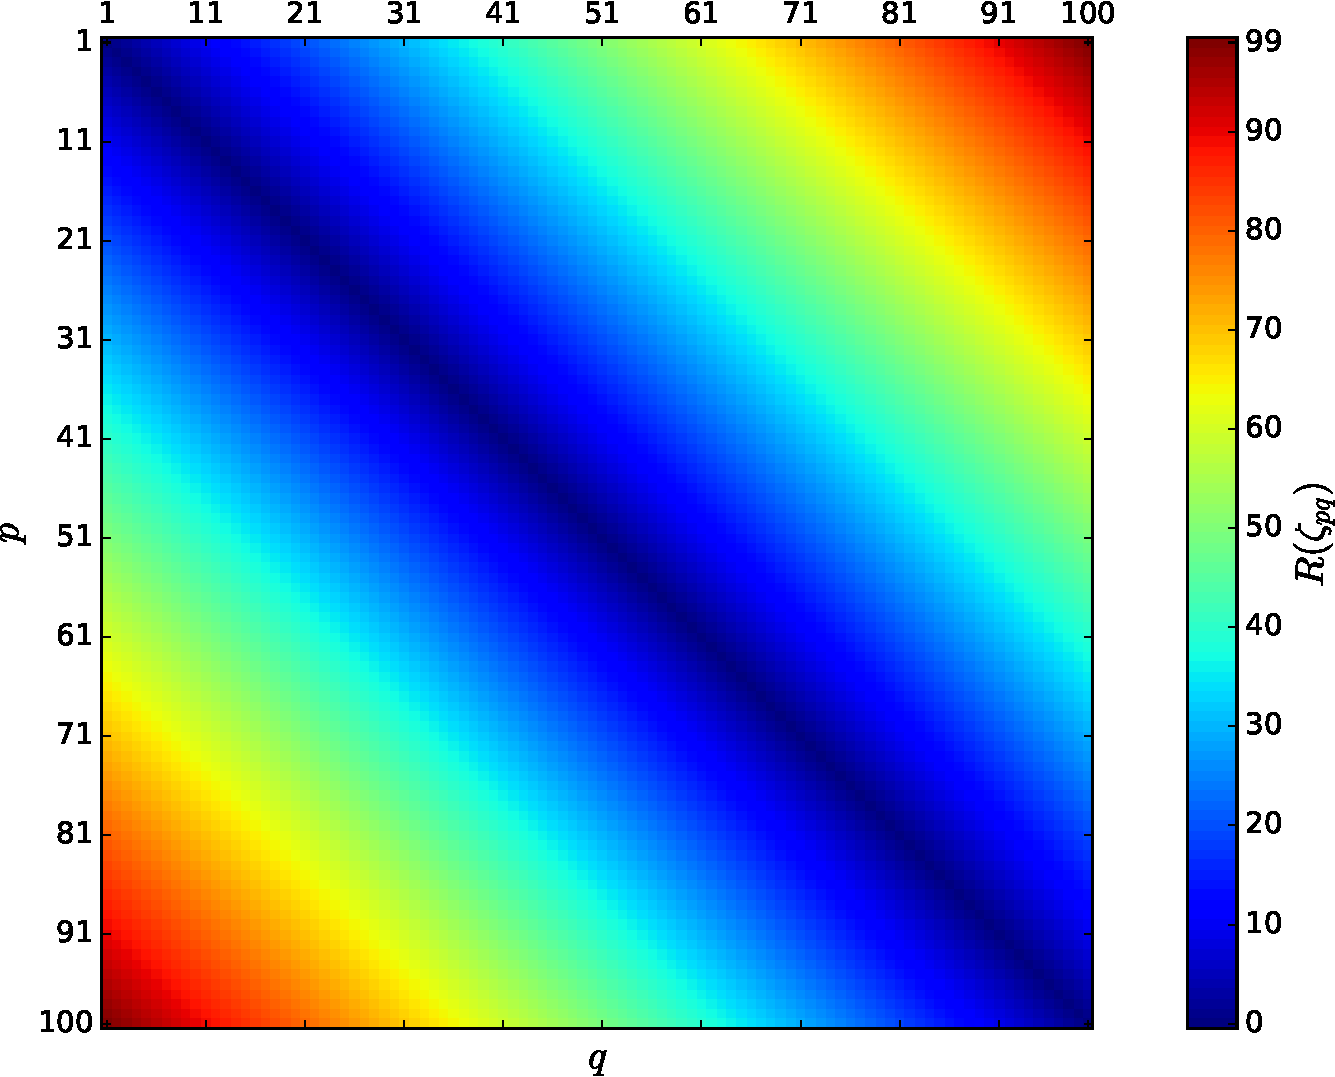
\includegraphics[width=0.33\textwidth]{./REG_phi.pdf}\label{fig:phase_pat_45}}
\caption{scenario. \label{fig:ghost_pattern_bas_45}}
\end{figure*}

If the mapping $\phi_{ij}$ is known and one is given one of the two antenna indexes that together form a redundant baseline as well as the redundant baseline index itself then it is possible 
to calculate the unknown antenna index. This can be calculated via the following two expressions:
\begin{equation}
\xi_{ij} = 
\begin{cases}
p~\textrm{if}~\exists! ~ p \in \mathbb{N} ~ s.t. ~(\phi_{pi} = j)\\
0~\textrm{otherwise}
\end{cases},
\end{equation}
and
\begin{equation}
\psi_{ij} = 
\begin{cases}
q~\textrm{if}~\exists! ~ q \in \mathbb{N} ~ s.t. ~(\phi_{iq} = j)\\
0~\textrm{otherwise}
\end{cases}
\end{equation}

We use $\xi_{ij}$ to retrieve the first antenna index of the composite antenna pair associated with a particular baseline if the index of the first antenna in the composite antenna pair and the unique redundant baseline index are known, while we use $\psi_{ij}$ to obtain 
a similar result; the second antenna index of the composite antenna pair. \textbf{NB::} I still need to plot $\zeta_{ij}$ for different antenna layouts.

If the array is redundant and the mapping $\phi_{ij}$ is known we can rewrite Eq.~\eqref{eq:vis_definition} as
\begin{equation}
\label{eq:vis_red}
d_{pq} = g_{p}\conj{g}_{q}y_{\phi_{pq}} + n_{pq}.
\end{equation}
Eq.~\eqref{eq:vis_red} can also be expressed in the following vector form 
\begin{equation}
\bd = \bv + \bn, 
\end{equation}
where 
\begin{eqnarray}
 \bd &=& [d_{pq}] \big \} ~ [pq] = 1\cdots B ~ (p<q),\nonumber\\
 \bv &=& [g_p y_{\phi_{pq}} \conj{g}_q]  \big \} ~ [pq] = 1\cdots B ~ (p<q),\nonumber\\
 \bn &=& [n_{pq}]  \big \} ~ [pq] = 1\cdots B ~ (p<q).\label{eq:vec_definitions}
\end{eqnarray}
In Eq.~\eqref{eq:vec_definitions}, $B$ denotes the number of baselines in the array.

We will be using the following SNR (signal-to-noise ratio) definition in this paper  
\begin{equation}
\textrm{SNR} = \frac{<\bv\odot\conj{\bv}>_{t,pq}}{<\bn\odot\conj{\bn}>_{t,pq}}, 
\end{equation}
where $<*>_{t,pq}$ denotes averaging over time and baselines and $\odot$ denotes the Hadamard product. The definition we use here is similar 
to the SNR definitions of \citet{Liu2010,Marthi2014}.

\bibliographystyle{mn2e}
\bibliography{paper}

\label{lastpage}

\end{document}
